\documentclass[11pt]{article}
\usepackage{amsmath,amsthm,verbatim,amssymb,amsfonts,amscd,graphicx,graphics}
\usepackage{hyperref,url,booktabs,amsfonts,nicefrac,microtype,amsmath,amssymb,mathtools,xcolor,graphicx,float,fancyhdr}
\newcommand{\var}{\textnormal{Var}}
\newcommand{\cov}{\textnormal{Cov}}
\newcommand{\corr}{\textnormal{Corr}}
\newcommand{\N}{\mathcal{N}}
\newcommand{\Bern}{\textnormal{Bern}}
\newcommand{\Bin}{\textnormal{Bin}}
\newcommand{\Beta}{\textnormal{Beta}}
\newcommand{\Mult}{\textnormal{Mult}} 
\newcommand{\Gam}{\textnormal{Gamma}}
\newcommand{\Geom}{\textnormal{Geom}}
\newcommand{\FS}{\textnormal{FS}}
\newcommand{\HGeom}{\textnormal{HGeom}}
\newcommand{\NBin}{\textnormal{NBin}}
\newcommand{\Expo}{\textnormal{Expo}}
\newcommand{\Pois}{\textnormal{Pois}}
\newcommand{\Unif}{\textnormal{Unif}}
\newcommand{\Laplace}{\textnormal{Laplace}}
\newcommand{\Logistic}{\textnormal{Logistic}}
\newcommand{\LN}{\mathcal{LN}}
\newcommand{\Cauchy}{\textnormal{Cauchy}}  
\usepackage{natbib}

\begin{document}

\title{CS265 Midway Check-in}
\author{Mali Akmanalp, Sophie Hilgard, Andrew Ross}
\maketitle

\section{Introduction}

Tuning data systems is hard. Even for systems like key-value stores that only
support the most minimal API (\texttt{put} and \texttt{get}), the possibilities
are often overwhelming. The developers of RocksDB \citep{rocksdb}, a popular
and powerful key-value store, freely admit \citep{rocksdb-tuning-guide} that
``configuring RocksDB optimally is not trivial,'' and that ``even [they] as
RocksDB developers don't fully understand the effect of each configuration
change.'' Configurations must be optimized with respect to a given
\textit{workload}, which is rarely known in advance, although it is sometimes
roughly characterizable. There has been recent work \citep{monkey} in
determining the optimal memory allocation for bloom filters in terms of
worst-case analysis and with respect to a number of basic workloads, but
realistic key-value store workloads, which have been analyzed e.g. for Facebook
\citep{characterizing-memcached}, exhibit enormous complexity with respect to
time, skewness, and key repeatability.

Our goal is somewhat ambitious -- we seek to optimize not just bloom filter
memory allocation but memory allocation across the entire key-value store (to
cache, memtable, bloom filters, and possibly even fence pointers), and to do it
with respect to workloads we model as stochastic processes.

\section{Workloads}

Here are a number of basic workloads we will use to generate queries to
benchmark our key-value store, both in RocksDB and in Python simulations. For
the simpler ones, we will also attempt to predict performance and derive
optimal parameters analyitically.

\textbf{Uniform} queries will be drawn uniformly from keys $k \in
\{0,1,...,K\}$, where $K$ is a maximum key (that we explore varying). When we
draw a particular key $k_i$ for the first time, we will insert it into the
database as a write, and subsequently we will treat it as a lookup. Later we
will explore making a certain fraction of these queries into updates. The case
of uniformly distributed queries is often one in which the cache is unhelpful,
but in practice is highly unrealistic. Nevertheless, this is the scenario that
many analyses assume for calculations of big O complexity.

\textbf{Round-Robin} queries are drawn deterministically using $k_i = (i \mod
K)$, i.e. we iteratively draw each key in sequence, then repeat. This is also a
bad case for our key-value store in its default configuration; the fact that a
key has been recently written or read is actually a contraindication we will
access it again.

\textbf{80-20} queries (which are considered in \citet{monkey}) are drawn such
that 20\% of the most recently inserted keys constitute 80\% of the lookups.
This is a simple model we will be able to analyze analytically that exhibits
more realistic skew.

\textbf{Zipf} queries are distributed according to a Zipf or zeta distribution,
where the probability of a given key $k$ is $\propto \frac{1}{k^s}$, where $s
\in (1, \infty)$ describes the skewness of the distribution; in the limit
$s=1$, it is uniform with $K=\infty$. Zipf-distributed queries are considered
in \citet{art} as another simple proxy for realistically skewed queries.

\textbf{Discover-Decay} queries are distributed according to the following
stochastic process, inspired by the Chinese Restaurant process \citep{crp} but
with time decay: with every passing time increment $\Delta t \sim
\Expo(\lambda_t)$, $n \sim \Pois(\lambda_n)$ new keys are written to the
key-value store, which each have an inherent popularity $\theta_i \sim
\Beta(a_\theta,b_\theta)$ with a random decay rate $\gamma_i \sim
\Beta(a_\gamma,b_\gamma)$ that determines the exponential rate at which they
become less popular. The probability of drawing each $k_i$ is given by
$p(k_i,t) \propto \theta_i\gamma_i^{t-t_i}$, where $t$ is the current time and
$t_i$ is when the key was inserted. At each time step we sample $N$ keys from
$\Mult(\{p(k_i,t)\})$. This stochastic process is somewhat arbitrary and we
hope to make it more realistic, but it does capture many of the essential
behaviors we know characterize key-value stores: new keys are constantly
inserted, some keys are much more popular than others, and the popularity of
most keys decays over time. The nonparametric nature of this stochastic process
may make inference difficult, and we also hope to enhance it to make it more
well-suited to realistic workloads (e.g. that exhibit daily periodicity), but
it seems much more able to simulate the richness of realistic queries than many
of the other models.

\section{Simulations}

We implemented a basic simulator of an LSM tree in Python \citep{lsmulator},
which simulates how an LSM tree with a variably sized cache, memtable, disk
layers, and bloom filters performs for an aribtrary sequence of queries. In
particular, we are able to simulate how often we are forced to access data on
disk (the main performance bottleneck for an LSM tree) and how often we can
respond with data in memory. So far, results suggest that the same LSM tree
architecture performs very differently under different query distributions
(Figure \ref{fig:sametree-diffqs}), and that different LSM tree architectures
perform very differently under the \textit{same} query distribution (Figure
\ref{fig:sameqs-difftree}). We are working on an optimization procedure to find
the best architecture for a given set of queries.

\begin{figure}[!htb]
\begin{center}
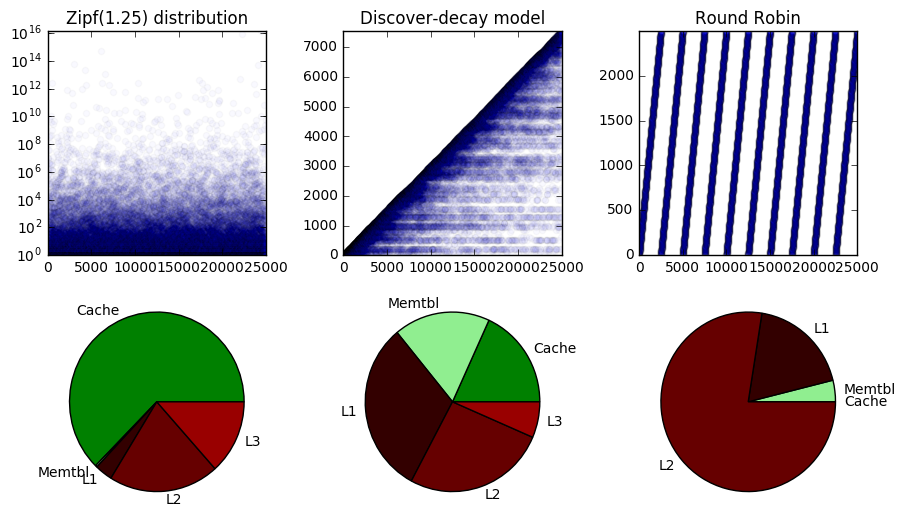
\includegraphics[width=\textwidth]{sametree-diffqs.png}
\end{center}
\caption{The same LSM tree architecture (a 25-element cache, 100-element
memtable, 5x layer ratio, and 10-bit bloom filters with 5 hash functions)
performs very differently for different query distributions. Memtable and cache
hits (in green) are fast, whereas accesses to the layers (in red) are slow. For
the Zipf workload, the cache is much more useful than the memtable, while the
situations are reversed for the Round-Robin workload. Both are useful in the
discover-decay case.}
\label{fig:sametree-diffqs}
\end{figure}

\begin{figure}[!htb]
\begin{center}
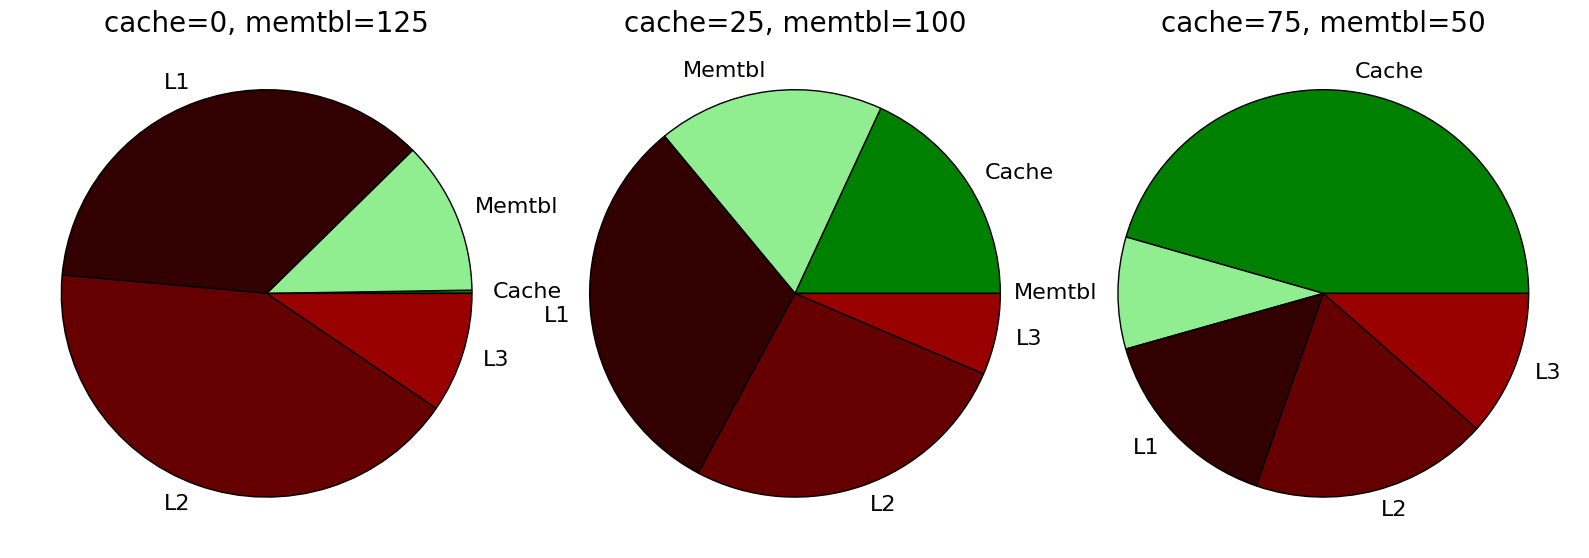
\includegraphics[width=\textwidth]{sameqs-difftree.png}
\end{center}
\caption{Performance results for different LSM tree architectures on the
discover-decay workload. Note that for this time-dependent workload, both the
cache and the memtable are useful, but finding the best ratio may require
optimization.}
\label{fig:sameqs-difftree}
\end{figure}

\section{Modeling}


\section{Benchmarking}

So far, we've succeeded in getting basic benchmarks for RocksDB running and
identifying which configuration parameters to vary

\bibliographystyle{named}
\small
\bibliography{bibliography}

\end{document}
